\documentclass[a4paper,nobind]{ociamthesis}  % no extra pages
% \documentclass[a4paper,twoside,hidelinks]{ociamthesis}  % uncomment lines 99 and 100 in ociamthesis.cls
% \documentclass[a4paper]{ociamthesis}  % one-sided binding


%%% PACKAGES %%%
\usepackage{tikz}
\usepackage{float}
\usepackage{lipsum}
\usepackage{xpatch}
\usepackage{custom}
\usepackage{subfig}
\usepackage{physics}
\usepackage{amsmath}
\usepackage{graphicx}
\usepackage{quantikz}
\usepackage{verbatim}
\usepackage{standalone}
\usepackage{circuitikz}
\usepackage{blochsphere}
\usepackage[parfill]{parskip}  % newline instead of indentation

%%% DRAFT VERSION %%%
\fancyfoot[C]{\emph{DRAFT Printed on \today}}  % draft in footer


%%% CORRECTIONS %%%
\correctionstrue  % comment out to remove corrections in blue
% \mccorrect{blah}  % word corrections
% \begin{mccorrection} ... \end{mccorrection}  % paragraph corrections


%%% Caption spacing
\setlength{\belowcaptionskip}{-8pt}


%%% GRAPHICS %%%
\graphicspath{{figures/}}

%%% BIBLIOGRAPHY %%%
\bibliographystyle{ref_style}

% uncomment for equations numbered per section rather than per chapter
% \numberwithin{equation}{subsection}


%%% TITLE PAGE %%%
\title{Diagrammatic Design of Ansätze for Quantum Chemistry}
\author{Ayman El Amrani}
\college{St. John's College}
\degree{Honour School of Chemistry}
\degreedate{Part II 2024}


%%% ========== BEGIN DOCUMENT ========== %%%
\begin{document}


%%% LINE SPACING CONFIG %%%
% \setlength{\textbaselineskip}{26pt}  % official line spacing
\setlength{\textbaselineskip}{22pt}  % official line spacing
\setlength{\frontmatterbaselineskip}{17pt plus1pt minus1pt} % roman pages
\setlength{\baselineskip}{\textbaselineskip}


%%% SECTION NUMBERING DEPTH CONFIG %%%
\setcounter{secnumdepth}{1}  % level that is numbered
\setcounter{tocdepth}{1}  % level that appears in table of contents


%%% ========== ROMAN PAGES ========== %%%
\begin{romanpages}
\maketitle

%%% DEDICATION %%%
\begin{dedication}
Pour ma mère et mon père. \\
% Merci de m'avoir amené jusqu'ici.
\end{dedication}

%%% ACKNOWLEDGEMENTS %%%
\begin{acknowledgements}
Thank you Thomas Cervoni for your constant motivation and support. \\
Thank you David Tew and Stefano Gogioso for your patient supervision. \\
Thank you Razin Shaikh, Boldizsár Poór, Richie Yeung and Harny Wang for always finding the time to answer my questions. \\
Thank you to my friends and family for supporting me during this unconvential Master's.
\end{acknowledgements}

%%% SUMMARY %%%
\begin{abstract}
	A central challenge in computational quantum chemistry is the accurate simulation of fermionic systems. At the heart of these calculations lies the need to solve the Schrödinger equation to determine the many-electron wavefunction. An exact solution to this problem scales exponentially with the number of electrons. Classical computers have no means by which to efficiently store the increasingly large wavefunctions, making this problem computationally intractable in many cases. In contrast, gate-based quantum computing presents a promising solution, offering the potential to represent electronic wavefunctions with polynomially scaling resources \cite{Burton2023}. In other words, quantum computers are a natural tool of choice for simulating processes that are inherently quantum \cite{Yeung2020}.

In the last two decades, many advancements in quantum computing have been made in both hardware and software, bringing us closer to being able to simulate molecular systems. Despite these advancements, we remain in the so-called Noisy Intermediate Scale Quantum (NISQ) era, characterised by challenges such as poor qubit fidelity, low qubit connectivity and limited coherence times. The NISQ era represents a transitional phase in quantum computing, where quantum devices are not yet error-corrected but are still capable of performing computations beyond the reach of classical computers. Overcoming the limitations of the NISQ era is crucial for realising the full potential of quantum computing in various fields, including quantum chemistry and materials science.

% The Variational Quantum Eigensolver (VQE) algorithm is a method used to estimate the ground state energy of a molecular Hamiltonian by preparing a trial wavefunction, calculating its energy, and optimising the wavefunction parameters classically until the energy converges to the best approximation for the ground state energy \cite{McClean2016}. It is recognised as a leading algorithm for quantum simulation on NISQ devices due to its reduced resource requirements in terms of qubit count and coherence time \cite{Kirby2020}.

This thesis concerns itself with the study of the excitation operators used to prepare parametrised quantum circuits representing fermionic wavefunctions, known as ansätze. We extend the work of Yeung \cite{Yeung2020} on Pauli gadgets and Yordanov \textit{et al} \cite{Yordanov2020} on fermionic excitation operators, concerning ourselves with two main questions: firstly, can we use the ZX calculus to gain insights into the structure of the unitary product ansatz in the context of variational algorithms for quantum chemistry? Secondly, in the context of NISQ devices, can we use these insights to build better ansätze with reduced circuit depth and more efficient resources?

Motivated by the structure of Pauli gadgets in the ZX calculus, we began this research with the goal of identifying a general structure for the excitation operators used to prepare fermionic ansätze in the ZX calculus. We anticipated that by identifying such structures, and identifying the rules describing their behaviour, we might discover novel ways of optimising ansätze representing fermionic wavefunctions. This led us to the work done by Yordanov \textit{et al}, which shows that excitation operators can be expressed in terms of controlled-rotations. Consequently, a significant portion of this thesis revolves around developing the diagrammatic techniques essential for replicating the findings of Yordanov \textit{et al} in the ZX calculus.

\begin{itemize}
    \item \textbf{Chapter \ref{background}} develops the mathematical foundation for simulating molecules on quantum computers.
    \item \textbf{Chapter \ref{zx-calculus}} introduces the generators of the ZX calculus and its rewrite rules.
    \item \textbf{Chapter \ref{pauli-gadgets}} introduces Pauli gadgets, the basic building blocks of fermionic ansätze, and their interaction with other quantum gates.
    \item \textbf{Chapter \ref{controlled-rotations}} explores controlled rotations in terms of phase polynomials.
    \item \textbf{Chapter \ref{excitation-operators}} applies the theory developed thus far to show how excitation operators can be expressed it terms of controlled rotations in the ZX calculus.
    \item \textbf{Chapter \ref{zxfermion}} introduces the software package ZxFermion that we built, demonstrating how it can be used to replicate the research done in this thesis.
\end{itemize}

\end{abstract}

\flushbottom  % align bottom of text of each page

%%% TABLE OF CONTENTS %%%
\tableofcontents

\end{romanpages}


%%% ========== CHAPTERS  ========== %%%

% BACKGROUND
\chapter{Background}%
\label{background}

% In this chapter, we will develop the mathematical foundation used to simulate fermionic systems on quantum computers and explain the process that we followed during this year's work. Starting with Electronic Structure Theory (\ref{electronic-structure-theory}), we will build up to Unitary Coupled Cluster theory and the Variational Quantum Eigensolver REF, which serves as the framework that this research revolves around.

% Fermionic states can generally be represented on a quantum computer in the occupation number representation (section REF(second-quantisation)). That is, the state of each qubit is taken to represent the occupancy of each spin orbital. By representing the fermionic creation and annhilation operators in terms of qubit operators in a way that preserves the fermionic anticommutation relations, we can express the molecular Hamiltonian in terms of qubit operations.

\section{Fundamentals of Quantum Computating}%
\label{quantum-computation}

The central concept that enables gate-based quantum computation to represrent exponentially scaling fermionic states with polynomially scaling quantum resources is its ability to encode and manipulate superpositions of states. In this section, we provide an introduction to qubits and basic quantum gates.

\subsection{Introduction to Qubits}

Classical computation encodes information using binary strings formed from the 0 and 1 computational basis. Thus, given $n$ classical bits, we can encode $2^n$ binary strings. In contrast, information on a quantum computer is encoded using two quantum states, corresponding to vectors in a two-dimensional complex Hilert space $\mathbb{C}$. The $\ket 0$ and $\ket 1$ states, known as the $Z$ computational basis, form the standard computational basis for encoding information on a quantum computer.

\begin{figure}[H]
    \centering
    \begin{minipage}{.45\textwidth}
        \centering
        \includezxdiagramtext{chapter-1/zero}{0.35}{\,\,\,
        \begin{pmatrix} 1 \\ 0 \end{pmatrix}}
    \end{minipage}%
    \begin{minipage}{0.45\textwidth}
        \centering
        \includezxdiagramtext{chapter-1/one}{0.35}{\,\,\,
        \begin{pmatrix} 0 \\ 1 \end{pmatrix}}
    \end{minipage}
    \caption{$Z$ computational basis states.}
    \label{z-eigenstates}
\end{figure}

An arbitrary qubit state $\ket\psi$ can be described as a complex linear combination of the computational basis states, $\ket\psi = \alpha\ket 0 + \beta\ket 1$, provided that the qubit state is normalised. In other words we require two complex numbers to describe an arbitrary qubit state. Since only the relative phase between the basis states is directly measureable, there is a redundancy in this description, allowing us to represent $\ket\psi$ using only three real numbers. Furthermore, since $\ket\psi$ is normalised, we can describe it using two real phases as follows $\ket\psi = \cos{\brac{\theta}{2}} + e^{i\phi} \sin{\brac{\theta}{2}} \ket 1$. This representation allows us to derive a three-dimensional representation for arbitrary qubit states known as the Bloch sphere. The Bloch sphere is a unit sphere in which opposite points correspond to mutually orthonal states. At one end of the $Z$ axis, we have the $\ket 0$ state, and at the other end, we have the $\ket 1$ state (Figure \ref{z-eigenstates}).

We could have chosen to form our computational basis with any pair of orthonormal states. For instance, we define the $X$ basis states as follows.

\begin{figure}[H]
    \centering
    \begin{minipage}{.45\textwidth}
        \centering
        \includezxdiagramtext{chapter-1/plus}{0.4}{\,\,\,
        \frac{\ket 0 + \ket 1}{\sqrt 2}}
    \end{minipage}%
    \begin{minipage}{0.45\textwidth}
        \centering
        \includezxdiagramtext{chapter-1/minus}{0.4}{\,\,\,
        \frac{\ket 0 - \ket 1}{\sqrt 2}}
    \end{minipage}
    \caption{Computational $X$ basis states.}
    \label{x-eigenstates}
\end{figure}

In theory, a qubit can exist in an infinite number of states, however, upon measuring with respect to a particular basis, the qubit state collapses into one basis state, or the other. This result gives rise to the \textit{no-cloning theorem}, which states that we cannot create indentical and independent copies of arbitrary qubit states, as this would first involve measuring that state.

\subsection{Multiple-Qubit States}

Let us now consider systems consisting of multiple qubits. Similarly to how $n$ classical bits give rise to $2^n$ binary strings, we have that, $n$ qubits give rise to $2^n$ basis states. These basis states are formed by taking the Kronecker product. For instance, a two-qubit system gives rise to the four following basis states.

\begin{figure}[H]
    \centering
    \begin{equation*}
        \ket{00} = \ket 0 \otimes \ket 0 \qquad
        \ket{01} = \ket 0 \otimes \ket 1 \qquad
        \ket{10} = \ket 1 \otimes \ket 0 \qquad
        \ket{11} = \ket 1 \otimes \ket 1
    \end{equation*}
    \caption{The four basis states associated with a two-qubit system.}
    \label{two-qubit-states}
\end{figure}

An arbitrary $n$-qubit \textit{state vector}, describing the state of the entire system, can be formed by taking a complex linear combination of the $2^n$ basis states. Therefore, in order to fully describe an arbitrary $n$-qubit state vector, we need to specify $2^n$ complex coefficients. In the case of a two-qubit system, we have the following.
\begin{gather*}
    \ket\psi =
    \alpha \ket{00} +
    \beta \ket{01} +
    \gamma \ket{10} +
    \delta \ket{11} \\
    \text{where} \,\,\,\, \alpha, \, \beta, \, \gamma, \, \delta \in \mathbb{C}
\end{gather*}

\newpage
\subsection{Introduction to Quantum Gates}%
\label{quantum-gates}

By definition, quantum gates correspond to unitary transformations, $U^{-1} = U^\dagger$ \cite{Nielsen2012}. In other words, any quantum gate corresponds to a square unitary matrix that conserves the complex inner product of the state it acts on. Consequently, quantum gates can be viewed as rotations of the qubit state vector in Hilbert space.

Let us now introduce the most fundamental quantum gates: the Pauli gates. The Pauli gates are described by the $2 \times 2$ Pauli matrices and rotate an arbitrary qubit state by $\pi$ radians about their respective axes.

\begin{figure}[H]
    \centering
    \begin{equation*}
        I = \begin{pmatrix} 1 & 0 \\ 0 & 1\end{pmatrix} \qquad
        X = \begin{pmatrix} 0 & 1 \\ 1 & 0\end{pmatrix} \qquad
        Y = \begin{pmatrix} 0 & -i \\ i & \,\,\,\,0\end{pmatrix} \qquad
        Z = \begin{pmatrix} 1 & \,\,\,0 \\ 0 & -1\end{pmatrix}
    \end{equation*}
    \caption{The Pauli matrices corresponding to the Pauli gates.}
    \label{pauli-matrices}
\end{figure}

The Pauli $X$ gate is the quantum analogue of the classical NOT gate in that it maps $\ket 0 \leftrightarrow \ket 1$. Importantly, the Pauli $X$ differs from its classical counterpart in that it can act on any arbitrary qubit state. Similarly, we have that the Pauli $Z$ gate maps $\ket + \leftrightarrow \ket -$, but can also act on any arbitrary qubit state.

The Hadamard gate is a member of the Clifford group that maps $\ket 0 \leftrightarrow \ket +$ and $\ket 1 \leftrightarrow \ket -$. Therefore, the Hadamard gate can be viewed as a rotation of the Bloch sphere $\pi$ radians about the line bisecting the $z$ and $x$ axes.

\begin{figure}[H]
    \centering
    \includezxdiagramtext{chapter-1/hadamard}{0.15}{
    \frac{1}{\sqrt 2} \begin{pmatrix} 1 & 1 \\ 1 & -1 \end{pmatrix}}
    \caption{Bloch sphere representation of the Hadamard gate.}
    \label{hadamard-definition}
\end{figure}

Since the Pauli gates and the Hadamard gate each correspond to unitary and Hermitian matrices, it follows that they are also self-inverse. Consequently, successively applying any of these gates is equivalent to applying the identity matrix $I$.

The R$_Z(\theta)$ and R$_X(\theta)$ rotation gates correspond to rotations of the Bloch sphere by some angle $\theta$ about the $Z$ and $X$ axes respectively.

\begin{figure}[H]
    \centering
    \begin{minipage}{0.45\textwidth}
        \centering
        \includezxdiagramtext{chapter-1/z_rotation}{0.4}{
        \begin{pmatrix} 1 & 0 \\ 0 & e^{i\theta} \\ \end{pmatrix}}
    \end{minipage}
    \begin{minipage}{0.45\textwidth}
        \centering
        \includezxdiagramtext{chapter-1/x_rotation}{0.35}{
        \begin{pmatrix}
              1 + e^{i\theta} & 1 - e^{i\theta} \\
              1 - e^{i\theta} & 1 + e^{i\theta}
        \end{pmatrix}}
    \end{minipage}
    \caption{Bloch sphere representations of arbitrary $Z$ and $X$ rotations.}
    \label{z-rotation-definition}
    \label{x-rotation-definition}
\end{figure}

\subsection{Multiple-Qubit Gates}

The CNOT gate is a two-qubit member of the Clifford group which we can use to entangle qubits. Consider a two-qubit state of the form $\ket \alpha \otimes \ket \beta$. Taking the first qubit ($\alpha$) to be the control, and the second qubit ($\beta$) to be the target, we define the CNOT gate as the gate that maps $\ket\alpha\otimes\ket\beta \rightarrow \ket\alpha\otimes\ket{\alpha\oplus\beta}$. That is, the CNOT gate applies the Pauli $X$ gate to the target qubit \textit{iff} the control qubit is in the $\ket 1$ state. The CNOT gate acts on the two-qubit basis states (\ref{two-qubit-states}) as follows.
\begin{equation*}
    \ket{00} \rightarrow \ket {00} \qquad
    \ket{01} \rightarrow \ket {01} \qquad
    \ket{10} \rightarrow \ket {11} \qquad
    \ket{11} \rightarrow \ket {10}
\end{equation*}
In this way the CNOT gate is the quantum generalisation of the classical XOR gate. We define the two matrices corresponding to the two CNOT gates, with the first qubit being the control and the second qubit being the target, and \textit{vice versa}.

\begin{figure}[H]
    \centering
    \begin{equation*}
    \text{CNOT}^{c=0}_{t=1} =
        \begin{pmatrix}
            1 & 0 & 0 & 0 \\
            0 & 1 & 0 & 0 \\
            0 & 0 & 0 & 1 \\
            0 & 0 & 1 & 0
        \end{pmatrix} \qquad
        %
        \text{CNOT}^{c=1}_{t=0} =
        \begin{pmatrix}
            1 & 0 & 0 & 0 \\
            0 & 0 & 0 & 1 \\
            0 & 0 & 1 & 0 \\
            0 & 1 & 0 & 0
        \end{pmatrix}
    \end{equation*}
    \caption{Matrix definitions of the CNOT gate.}
    \label{cnot-definition}
\end{figure}

The CNOT gate can be used to entangle two qubits when the control qubit exists in a superposition of states. For instance, applying CNOT gate to the $\ket{+0}$ state, letting the first qubit be the control qubit ($\ket +$), yields the following Bell state.
\begin{equation*}
    \text{CNOT} \ket{+ \, 0} = \frac{\ket{00} + \ket{11}}{\sqrt 2}
\end{equation*}


\section{\label{electronic-structure-theory}Electronic Structure Theory}

\subsection{Electronic Structure Problem}

% References: \cite{Atilla1996}

The main interest of electronic structure theory is finding approximate solutions to the eigenvalue equation of the full molecular Hamiltonian. Specifically, we seek solutions to the non-relativistic time-independent Schrödinger equation.

The full molecular Hamiltonian describes all of the interactions within a system of $N$ interacting electrons and $M$ nuclei. We are able to simplify the problem to an electronic one using the Born-Oppenheimer approximation. Motivated by the large difference in mass of electrons and nuclei, we can approximate nuclei as stationary on the timescale of electronic motion such that the electronic wavefunction depends only parametrically on the nuclear coordinates. Within this approximation, the nuclear kinetic energy term can be neglected and the nuclear repulsive term is considered to be constant. Following this, we obtain the electronic Hamiltonian for $N$ electrons.

\begin{figure}[H]
\begin{equation*}
    H =
    - \sum_{i=1}^{N} \frac{1}{2} \nabla^{2}_{i}
    - \sum_{i=1}^{N} \sum_{j=1}^{M} \frac{Z_j}{|r_{i} - R_{j}|}
    + \sum_{i=1}^{N} \sum_{j>i}^{N} \frac{1}{|r_{i} - r_{j}|}
\end{equation*}
\caption{Electronic molecular Hamiltonian in atomic units.}
\end{figure}

The first term corresponds to the kinetic energy of the $N$ electrons in the system, the second term corresponds to the pairwise attractive Coulombic interactions between the $N$ electrons and $M$ nuclei and the final term corresponds to the repulsive Coulombic interactions between $N$ electrons in the system. Throughout the remainder of this text, we concern ourselves only with the electronic Hamiltonian, simply referring to it as the Hamiltonian, $H$. The solution to the eigenvalue equation involving the electronic Hamiltonian is the electronic wavefunction, which depends only parametrically on the nuclear coordinates. It is solved for fixed nuclear coordinates, such that different arrangements of nuclei yields different functions of the electronic coordinates. The total molecular energy can be calculated by solving the electronic Schrödinger equation and including a constant nuclear term.

% \begin{equation*}
%     E_\text{total} = E_\text{elec} + \sum_{i=1}^{M} \sum_{j>i}^{M} \frac{Z_{i} Z_{j}}{|R_{i} - R_{j}|}
% \end{equation*}

\subsection{Many-Electron Wavefunctions}%
\label{many-electron-wavefunctions}

The many-electron wavefunction, which describes all the electrons in given molecular system, must satisfy the Pauli principle. This is an independent postulate of quantum mechanics that requires the many-electron wavefunction to be antisymmetric with respect to the exchange of any two fermions.

A spatial molecular orbital is defined as a one-particle function of the position vector, spanning the whole molecule. The spatial orbitals form an orthonormal set $\{\psi_i(\mathbf{r})\}$, which if complete can be used to expand any arbitrary single-particle molecular wavefunction, that is, an arbitrary single-particle function of the position vector. In practice, only a finite set of such orbitals is available to us, spanning only a subspace of the complete space. Hence, wavefunctions expanded using this finite set are described as being `exact' only within the subspace that they span.

We now introduce the spin orbitals $\{\phi_i(\mathbf{x})\}$, that is, the set of functions of the composite coordinate $\mathbf{x}$, which describes both the spin and spatial distribution of an electron. Given a set of $K$ spatial orbitals, we can construct $2K$ spin orbitals by taking their product with the orthonormal spin functions $\alpha(\omega)$ and $\beta(\omega)$. Whilst the Hamiltonian operator makes no reference to spin, it is a necessary component when constructing many-electron wavefunctions in order to correctly antisymmetrise the wavefunction with respect to fermion exchange. Constructing the antisymmetric many-electron wavefunction from a finite set of spin orbitals amounts to taking the appropriate linear combinations of symmetric products of $N$ spin orbitals. A general procedure for this is achieved by constructing a Slater determinant from the finite set of spin orbitals, where each row relates to the electron coordinate $\mathbf{x_n}$ and each column corresponds to a particular spin orbital $\phi_i$ \cite{Atilla1996}. 

\begin{figure}[H]
\centering
\begin{equation*}
\psi(\mathbf{x}_1, \mathbf{x}_2) =
%
\frac{1}{\sqrt{N!}} \begin{vmatrix}
\phi_i (\mathbf{x}_1) & \phi_j (\mathbf{x}_1) & \dots & \phi_k (\mathbf{x}_1) \\
\phi_i (\mathbf{x}_2) & \phi_j (\mathbf{x}_2) & \dots & \phi_k (\mathbf{x}_2) \\
\vdots & \vdots &   & \vdots \\
\phi_i (\mathbf{x}_N) & \phi_j (\mathbf{x}_N) & \dots & \phi_k (\mathbf{x}_N)
\end{vmatrix}
\end{equation*}
\caption{Slater determinant representing an antisymmetrised $N$-electron wavefunction.}
\end{figure}

% Since exchanging any two rows or columns of a determinant changes its sign, Slater determinants satisfy the Pauli principle by definition. Slater determinants constructed from orthonormal spin orbitals are themselves normalised and $N$ electron Slater determinants constructed from different orthonormal spin orbitals are orthogonal to one another \cite{Atilla1996}.

By constructing Slater determinants and antisymmetrising the many-electron wavefunction to meet the requirements of the Pauli principle, we have incorporated exchange correlation, in that, the motion of any two electrons with parallel spins is now correlated \cite{Atilla1996}.

The Hartree-Fock method yields a set of orthonormal spin orbitals, which when used to construct a single Slater determinant, gives the best variational approximation to the ground state of a system \cite{Atilla1996}. By treating electron-electron repulsion in an average way, the Hartree-Fock approximation allows us to iteratively solve the Hartree-Fock equation for spin orbitals until they become the same as the eigenfunctions of the Fock operator. This is known as the Self-Consistent Field (SCF) method and is an elegant starting point for finding approximate solutions to the many-electron wavefunction.

% \begin{figure}[H]
% \centering
% \begin{equation*}
% \left[
% -\frac{1}{2}\nabla^2 - \sum_{A=1}^M \frac{Z_A}{r_{i_A}} + \nu^\text{HF}(i)
% \right]
% \phi_i(\mathbf x_i) = \varepsilon \phi_i(\mathbf x_i)
% \end{equation*}
% \caption{Hartree-Fock equation used in the Self-Consistent Field method.}
% \end{figure}

% For an $N$ electron system, and given a set of $2K$ Hartree-Fock spin orbitals, where $2K > N$, there exist many different single Slater determinants. The Hartree-Fock groundstate being one of these. The remainder are excited Slater determinants, recalling that all of these must be orthogonal to one-another. By treating the Hartree-Fock ground state as a reference state, we can describe the excited states relative to the reference state, as single, double, \dots, N-tuple excited states \cite{Atilla1996}.

\subsection{\label{second-quantisation}Second Quantisation}

% References: \cite{Helgaker2000}, \cite{Fetter1972}

In second quantisation, both observables and states are represented by creation and annihilation operators. Unlike the standard formulation of quantum mechanics, these operators inherently incorporate Bose or Fermi statistics, eliminating the need to track symmetrised or antisymmetrised products of single-particle wavefunctions. Put differently, the antisymmetry of an electronic wavefunction follows from the algebra of these operators, which greatly simplifyies the discussion of many identical interacting fermions \cite{Helgaker2000}, \cite{Fetter1972}.

The Fock space is a linear abstract vector space spanned by $N$ orthonormal occupation number vectors, each representing a single Slater determinant \cite{Helgaker2000}. Hence, given a basis of $N$ spin orbitals we can construct $2^N$ single Slater determinants, each corresponding to a single occupation number vector in the full Fock space. The occupation number representation of fermionic states is succinctly denoted in Dirac notation as below, where the occupation number $f_j$ is 1 if spin orbital $j$ is occupied, and 0 if spin orbital $j$ is unnoccupied.
\begin{equation*}
    \ket\psi = \ket{f_{n-1} \,\, f_{n-2} \dots f_{1} \,\, f_{0}} \qquad \text{where } f_{j} \in {0, 1}
\end{equation*}
Whilst there is a one-to-one mapping between Slater determinants with canonically ordered spin orbitals and the occupation number vectors in the Fock space, it is important to distinguish between the two since, unlike the Slater determinants, the occupation number vectors have no spatial structure and are simply vectors in an abstract vector space \cite{Helgaker2000}.

Operators in second quantisation are constructed from the creation and annihilation operators $a_j^\dagger$ and $a_j$, where the subscripts $i$ and $j$ denote the spin orbital. $a_j^\dagger$ and $a_j$ are one another's Hermitian adjoints, and are not self-adjoint \cite{Helgaker2000}. Due to the fermionic exchange anti-symmetry imposed by the Pauli principle, the action of the creation and annhilation operators introduces a phase to the state that depends on the parity of the spin orbitals preceding the target spin orbital. This phase factor is automatically kept track of by the creation and annhilation operators' anticommutation relations \cite{Helgaker2000}.
\begin{figure}[H]
    \centering
    \begin{equation*}
        \{ \hat a_{j}, \hat a_{k} \} = 0 \qquad \qquad
        \{ \hat a_{j}^{\dagger}, \hat a_{k}^{\dagger} \} = 0 \qquad
        \{ \hat a_{j}, \hat a_{k}^{\dagger} \} = \delta_{jk} \hat{1}
    \end{equation*}
    \caption{Anticommutation relations of the creation and annhilation operators.}
    \label{anticommutation-relations}
\end{figure}
The Hamiltonian in second quantisation can be expressed as follows, where the one-body matrix element $h_{ij}$ corresponds to the kinetic energy of an electron and its interaction energy with the nuclei, and the two-body matrix element $h_{ijkl}$ corresponds to the repulsive interaction between electrons $i$ and $j$.
\begin{equation*}
    \hat H =
    \sum_{ij} h_{ij} a^\dagger_i a_j +
    \frac{1}{2} \sum_{ijkl} h_{ijkl} a^\dagger_i a^\dagger_j a_k a_l +
    h_\text{Nu}
\end{equation*}
These matrix elements are then computed classically, allowing us to simulate only the inherently quantum aspects of the problem on a quantum computer.
\begin{gather*}
h_{ij} = \int^\infty_{-\infty} \psi^*_{i(x_1)} \left( - \frac{1}{2} \nabla^2 + \hat V_{(x_1)} \right) \psi_{j(x_1)} \,\, d^3 x_1 \\[3ex]
%
h_{ijkl} = \int^\infty_{-\infty} \int^\infty_{-\infty} \psi^*_{i(x_1)} \psi^*_{j(x_2)} \left( \frac{1}{|x_1 - x_2|} \right) \psi_{k(x_2)} \psi_{l(x_1)} \,\, d^3 x_1 d^3 x_2
\end{gather*}

\section{The Variational Quantum Eigensolver}%
\label{vqe}

In this chapter, we introduce the \textit{Variational Quantum Eigensolver (VQE)} algorithm, a particular class of variational quantum algorithms used to estimate the ground state energy of molecular systems. The research presented in this thesis is conducted within this framework. As providing an overview of the VQE algorithm, we will introduce the fundamentals of quantum computing and the \textit{Unitary Coupled Cluster (UCC) ansatz} used to represent fermionic wavefunctions on quantum devices.

The VQE algorithm consists of a quantum subroutine, a \textit{Parametrised Quantum Circuit (PQC)}, that implements some UCC ansatz, and a classical subroutine that classically optimises the UCC ansatz until it converges to the best approximation of the true ground state. PQCs are similar to classical neural networks in concept, but by definition, correspond to $2^n \times 2^n$ unitary maps, where $n$ is the number of qubits, and hence have the same number of inputs as outputs \cite{Yeung2020}.

The input state for the PQC is the reference state that the UCC operator $U(\bm\theta)$ acts on, which in the case of the single Slater determinant Hartree-Fock state, is encoded as a pure quantum state $\ket{\psi_0}$. The output of the PQC is then an entangled state, that is, some linear combination of vectors in the Fock space, that captures the correlation present in true ground state of the molecular system of interest.

Upon measuring the PQC output state, it collapses into a single vector in the Fock space, with a probability defined by that vector's weight in the UCC ansatz. The quantum subroutine computes the energy expectation value of the UCC ansatz via a quantum circuit consisting of the PQC and the Hamiltonian for the system.

\includezxdiagram{chapter-1/expectation}{0.7}
\begin{equation*}
    E(\bm\theta) = \bra{0} U^\dagger(\bm\theta) H U(\bm\theta) \ket{0} 
\end{equation*}

For the purposes of this thesis, we are interested in a variant of the VQE algorithm developed by Burton \textit{et al} \cite{Burton2023} known as the \textit{Discretely and Continuously Optimised Variational Quantum Eigensolver (DISCO-VQE)}. We implement a fermionic state on a quantum device as a sequence of quantum gates representing unitary excitation operators that act on some reference state. The DISCO-VQE algorithm then finds approximate solutions to the fermionic ground state by both (\textit{discretely}) optimising the sequence of fermionic excitation operators, chosen from a finite operator pool, and (\textit{continuously}) optimising their parameters. This allows us to parametrically explore the Hilbert space of possible quantum states until we find a good approximation of the true fermionic ground state \cite{Taube2006}. The DISCO-VQE algorithm, therefore, discovers accurate representations of the fermionic UCC wavefunction using a minimal number of parameters \cite{Burton2023}.

%%%

\subsection{Unitary Coupled Cluster Ansatz}%
\label{unitary-coupled-cluster-ansatz}

As suggested by Peruzzo \textit{et al} \cite{Peruzzo2014}, the UCC formulation of a wavefunction can be efficiently implemented on a quantum device in terms of quantum gates, whose implementation we refer to as the UCC ansatz $\ket{\psi(\bm\theta)}$. In other words, the UCC ansatz corresponds to some unitary excitation operator $U(\bm\theta)$ that acts on a reference state, usually a single reference Slater determinant Hartree-Fock state $\ket{\psi_0}$ obtained via the self-consistent field method.
\begin{equation*}
    \ket{\psi(\bm\theta)} = U(\bm\theta) \ket{\psi_0} =
    e^{\hat T(\bm\theta) - \hat T^\dagger(\bm\theta)} \ket{\psi_0}
\end{equation*}

The operator $\hat T(\bm\theta)$ is a linear combination of fermionic excitation operators, parametrised by coupled cluster amplitudes $\bm\theta$. The exponential of the anti-Hermitian operator $\hat T(\bm\theta) - \hat T^\dagger(\bm\theta)$ is therefore, by definition, unitary. 
\begin{equation*}
\hat T(\bm{\theta}) - \hat T^{\dagger}(\bm{\theta}) =
\sum_{i, a} \theta^a_i (a^\dagger_i a_a - a^\dagger_a a_i) + 
\sum_{i, j, a, b} \theta^{ab}_{ij} (a^\dagger_i a^\dagger_j a_a a_b - a^\dagger_a a^\dagger_b a_i a_j) + \dots
\end{equation*}

Where $i, j$ indexes occupied spin orbitals and $a, b$ indexes virtual, or unoccupied, spin orbitals. The resulting unitary operator $U(\bm\theta)$ cannot be directly implemented on a quantum computer since the terms of the excitation operator do not commute. Instead, we must invoke the Trotter formula to approximate the unitary. Taking a single Trotter step $\rho=1$, since our focus is on the NISQ setting \cite{Cowtan2020}, we define the UCC ansatz as the following product of $k$ parametrised unitary operators.

\begin{figure}[H]
    \centering
    \begin{equation*}
        \ket{\psi(\bm\theta)} = \prod_{m=1}^k U_m(\theta_m) \ket{\psi_0} \qquad
        U_m(\theta_m) = e^{\theta_m (\tau_m - \tau_m^\dagger)}
    \end{equation*}
    \caption{Parametrised $k$-UCC ansatz.}
\end{figure}

Where $m$ indexes all possible excitations and $\tau_m - \tau_m^\dagger$ corresponds to anti-Hermitian fermionic excitation operators in second quantisation. For the remainder of this thesis, we will refer to fermionic excitation operators $U_m(\theta_m)$ as the the exponentials of these anti-Hermitian operators. As these fermionic excitation operators derive from second-quantised operators, they preserve the fermionic anti-symmetry and particle number of the reference state.

The operators are then mapped to quantum gates (see Chapter \ref{excitation-operators}) before being implemented on a quantum device. It has been shown by Evangelista \textit{et al} \cite{Evangelista2019} that the UCC ansatz can exactly parametrise any state. Within the DISCO-VQE framework, we consider only generalised \textit{single} (one-body) and \textit{double } (two-body) fermionic excitation (operators), which as shown by Evangelista \textit{et al} \cite{Evangelista2019} achieves universality provided that we combine enough suitably-ordered one-body and two-body excitation operators \cite{Burton2023}. In other words, the UCCSD ansatz is sufficient to represent any vector in the Hilbert space.

\begin{figure}[H]
    \centering
    \begin{equation*}
    \hat T(\bm{\theta}) - \hat T^{\dagger}(\bm{\theta}) =
    \sum_{i, a} \theta^a_i (a^\dagger_i a_a - a^\dagger_a a_i) + 
    \sum_{i, j, a, b} \theta^{ab}_{ij} (a^\dagger_i a^\dagger_j a_a a_b - a^\dagger_a a^\dagger_b a_i a_j)
    \end{equation*}
    \caption{Truncated operator containing only \textit{single} and \textit{double} excitations.}
\end{figure}


% ZX CALCULUS
\chapter{ZX Calculus}%
\label{zx-calculus}

The ZX calculus is a diagrammatic language for reasoning about quantum processes LALALA

We will then introduce the rewrite rules... that come equipped with the ZX calculus. These rules extend the ZX calculus from notation into a language.

Notation
- flow of time goes from left to right
- global scalar factor


Note that in this text, we will interpret the flow of time from left to right.
Whilst we obtain the correct states, we obtain the wrong scalar factor. For the remainder of this thesis, we will ignore global non-zero scalar factors. Hence, equal signs should be interpreted as `equal up to a global phase'.

All the diagrams in this chapter also hold for the colour-swapped counterparts.

\section{Generators}

Let us start by introducing two generators: the Z Spider and the X Spider. By sequentially or horizontally composing these generators, we can construct undirected multigraphs known as ZX diagrams. That is, graphs that allow multiple edges between vertices \cite{Wetering2020}. A ZX diagram is one level of abstraction above a quantum circuit. It represents the linear map between some input state and some output state.

Z Spiders are defined with respect to the $Z$ eigenbasis such that a Z Spider with any number of inputs and outputs has the following interpretation as a linear map. Note that in this text, we will interpret the flow of time from left to right.
\begin{figure}[H]
\centering
\includezxdiagram{figures/chapter-2/z_spider}{0.21}{\,
    \ket{0}^{\otimes m} \bra{0}^{\otimes n} + e^{i\alpha}
    \ket{1}^{\otimes m} \bra{1}^{\otimes n}}
\caption{Interpretation of Z Spider as a linear map.}
\end{figure}
Similarly, X Spiders, which are defined with respect to the $X$ eigenbasis, are interpreted as the following linear map.
\begin{figure}[H]
\centering
\includezxdiagram{figures/chapter-2/x_spider}{0.21}{\,
    \ket{+}^{\otimes m} \bra{+}^{\otimes n} + e^{i\alpha}
    \ket{-}^{\otimes m} \bra{-}^{\otimes n}}
\caption{Interpretation of X Spider as a linear map.}
\end{figure}

We can recover the $\ket 0$ eigenstate with an X Spider that has a phase of zero, or the $\ket 1$ eigenstate with an X Spider that has a phase of $\pi$.
\begin{figure}[H]
\centering
\begin{minipage}{.4\textwidth}
    \centering
    \includezxdiagram{figures/chapter-2/zero_state}{0.17}{\,
        \ket + + \ket - = \sqrt{2} \ket 0}
    \caption{$\ket 0$ eigenstate}
\end{minipage}%
\begin{minipage}{.4\textwidth}
    \centering
    \includezxdiagram{figures/chapter-2/one_state}{0.17}{\,
    \ket + - \ket - = \sqrt{2} \ket 1}
    \caption{$\ket 1$ eigenstate}
\end{minipage}
\end{figure}

Likewise, we have the $\ket +$ and $\ket -$ basis states from the corresponding Z Spider
\begin{figure}[H]
\centering
\begin{minipage}{.4\textwidth}
    \centering
    \includezxdiagram{figures/chapter-2/plus_state}{0.17}{\,
        \ket 0 + \ket 1 = \sqrt{2} \ket +}
    \caption{$\ket +$ eigenstate}
\end{minipage}%
\begin{minipage}{.4\textwidth}
    \centering
    \includezxdiagram{figures/chapter-2/minus_state}{0.17}{\,
    \ket 0 - \ket 1 = \sqrt{2} \ket -}
    \caption{$\ket -$ eigenstate}
\end{minipage}
\end{figure}

Importantly, whilst we recover the correct states, we obtain the wrong scalar factor. For the remainder of this thesis, we will ignore global non-zero scalar factors. Hence, equal signs should be interpreted as `equal up to a global phase'.

Single qubit rotations in the $X$ basis are represented by a Z Spider with a single input and a single output, whilst single qubit rotations in the $X$ basis are represented by the corresponding $X$ spider.
\begin{figure}[H]
\centering
\includezxdiagram{figures/chapter-2/z_rotation}{0.11}{
    \ket{0} \bra{0} + e^{i\alpha} \ket{1} \bra{1} = 
    \begin{pmatrix} 1 & 0 \\ 0 & e^{i\alpha} \end{pmatrix}
} \\[1ex]
\includezxdiagram{figures/chapter-2/x_rotation}{0.11}{
    \ket{+} \bra{+} + e^{i\alpha} \ket{-} \bra{-} = 
    \frac{1}{2}
    \begin{pmatrix}
        1 + e^{i\alpha} & 1 - e^{i\alpha} \\
        1 - e^{i\alpha} & 1 + e^{i\alpha}
    \end{pmatrix}
}
\caption{Arbitrary single qubit rotations in the $Z$ and $X$ bases.}
\end{figure}

Recall single qubit rotations can be interpreted as rotations of the qubit state vector inside the Bloch sphere.
\begin{figure}[H]
\centering
\begin{minipage}{.4\textwidth}
    \centering
    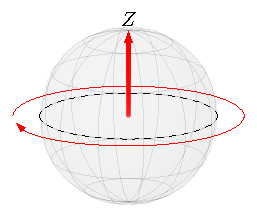
\includegraphics[width=0.5\textwidth]{chapter-1/z_rotation}
    \caption{lorum ipsum}
\end{minipage}%
\begin{minipage}{.4\textwidth}
    \centering
    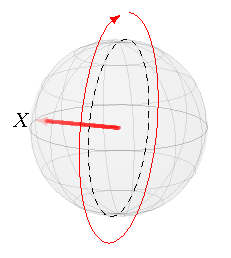
\includegraphics[width=0.46\textwidth]{chapter-1/x_rotation}
    \caption{lorum ipsum}
\end{minipage}
\end{figure}


The Pauli $Z$ and Pauli $X$ matrices are obtained by setting $\alpha = \pi$.
\begin{figure}[H]
\centering
\includezxdiagram{figures/chapter-2/pauli_z}{0.11}{
    \ket{0} \bra{0} + e^{i\pi} \ket{1} \bra{1} = 
    \begin{pmatrix} 1 & \,\,0 \\ 0 & -1 \end{pmatrix}
} \\[1ex]
\includezxdiagram{figures/chapter-2/pauli_x}{0.11}{
    \ket{+} \bra{+} + e^{i\pi} \ket{-} \bra{-} = 
    \begin{pmatrix} 0 & 1 \\ 1 & 0 \end{pmatrix}
}
\caption{Arbitrary single qubit rotations in the $Z$ and $X$ bases.}
\end{figure}

%%%

\subsubsection{Only Connectivity Matters}


\subsubsection{Composition}
We can take the matrix product by sequentially composing spiders in a ZX diagram. Note that the order of operation for matrix multiplication is from right to left, the opposite of the ZX diagram as we have defined it.

\begin{figure}[H]
    \centering
    \includezxdiagram{chapter-2/sequential}{0.27}{
        \begin{pmatrix} 1 & 0 \\ 0 & e^{i\gamma} \end{pmatrix}
        \begin{pmatrix}
            1 + e^{i\beta} & 1 - e^{i\beta} \\
            1 - e^{i\beta} & 1 + e^{i\beta}
        \end{pmatrix}
        \begin{pmatrix} 1 & 0 \\ 0 & e^{i\alpha} \end{pmatrix}}
\end{figure}

Alternatively, we could have chosen to compose the spider in parallel, resulting in the tensor product.
\begin{figure}[H]
    \centering
    \includezxdiagram{chapter-2/parallel}{0.11}{
        \begin{pmatrix} 1 & 0 \\ 0 & e^{i\alpha} \end{pmatrix} \otimes
        \begin{pmatrix}
            1 + e^{i\beta} & 1 - e^{i\beta} \\
            1 - e^{i\beta} & 1 + e^{i\beta}
        \end{pmatrix}}
\end{figure}

For instance, the CNOT gate, which is defined as the following diagram
...

Can be decomposed into matrix products and tensor products of spiders.
\begin{figure}[H]
    \centering
    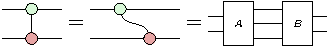
\includegraphics[width=0.65\textwidth]{chapter-2/cnot_def}
\end{figure}

\begin{figure}[H]
    \centering
    \includezxdiagram{chapter-2/A_def}{0.33}{
        \begin{pmatrix}
            1 & 0 \\
            0 & 0 \\
            0 & 0 \\
            0 & 1 \\
        \end{pmatrix} \otimes
        \begin{pmatrix} 1 & 0 \\ 0 & 1 \end{pmatrix}}
\end{figure}

\begin{figure}[H]
    \centering
    \includezxdiagram{chapter-2/B_def}{0.33}{
        \begin{pmatrix} 1 & 0 \\ 0 & 1 \end{pmatrix} \otimes 
        \frac{1}{\sqrt 2}
        \begin{pmatrix} 1 & 0 & 0 & 1 \\ 0 & 1 & 1 & 0 \end{pmatrix}}
\end{figure}

\begin{figure}[H]
    \centering
    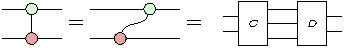
\includegraphics[width=0.65\textwidth]{chapter-2/cnot_def2}
\end{figure}

\begin{figure}[H]
\centering
\begin{minipage}{.4\textwidth}
    \centering
    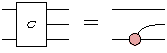
\includegraphics[width=0.80\textwidth]{chapter-2/C_def}
\end{minipage}%
\begin{minipage}{.4\textwidth}
    \centering
    \includegraphics[width=0.80\textwidth]{chapter-2/D_Def}
\end{minipage}
\end{figure}


\section{Rewrite Rules}%
\label{rewrite-rules}

% In this section, we will introduce the set of rules that transforms the ZX calculus from simply notation into a language \cite{Wetering2020}.

\notation{We will refer to the rules by some shorthand notation above equal signs. Note that this could refer to applying the rule in either direction.}

\subsection{Spider Fusion}%
The most fundamental rule of the ZX calculus is the \textit{spider fusion rule} (\textit{f}). It states that spiders of the same colour connected by one or more wires fuse and their phases add modulo $2\pi$ \cite{Wetering2020}.

\begin{figure}[H]
    \centering
    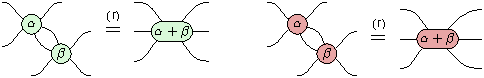
\includegraphics[width=0.75\textwidth]{chapter-2/fusion}
    \caption{Spider fusion rule for $Z$ spiders (left) and $X$ spiders (right).}
    \label{spider-fusion}
\end{figure}

It is the generalisation of adding the phases of successive rotations of the Bloch sphere. We can use this rule to show that $Z$ rotations commute through CNOT controls, and that $X$ rotations commute through CNOT targets.

% \vspace{5pt}
\includezxdiagram{chapter-2/cnot_commutation}{0.8}

%%%

\subsection{Identity Removal}%

The \textit{identity rule} (\textit{id}) states that any two-legged spider with no phase ($\alpha = 0$) is equivalent to a rotation by 0 radians, or identity.

\begin{figure}[H]
    \centering
    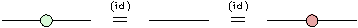
\includegraphics[width=0.6\textwidth]{chapter-2/identity}
    \caption{Identity removal rule.}
    \label{identity}
\end{figure}

Combining this with the spider fusion rule (\ref{spider-fusion}), we see that two successive rotations with opposite phases is equivalent to an empty wire.

\includezxdiagram{chapter-2/cancelling_rotations}{0.7}

%%%

\subsection{State Copy and $\pi$ Copy Rules}%

We can depict the $Z$ and $X$ eigenstates by assigning a phase to a $Z$ or an $X$ spider, respectively, through a Boolean variable $a$ (0 or 1) multiplied by $\pi$ \cite{Wetering2020}.

\includezxdiagramtext{chapter-2/boolean_x}{0.075}{
\ket 0 \text{ where $a = 0$ and }
\ket 1 \text{ where $a = 1$}}
%
\includezxdiagramtext{chapter-2/boolean_z}{0.075}{
\ket + \text{ where $a = 0$ and }
\ket - \text{ where $a = 1$}}

The $\pi$ \textit{copy rule} (\textit{c}) states that when a Pauli $Z$ or Pauli $X$ gate is pushed through a spider of the opposite colour, it is copied on all other legs and negates the spider's phase. A similar \textit{state copy rule} (\textit{c}) applies to the $Z$ and $X$ eigenstates.

\begin{figure}[H]
    \centering
    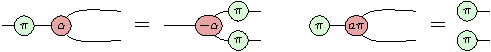
\includegraphics[width=0.9\textwidth]{chapter-2/pi_state_copy}
    \caption{$\pi$ copy (left) and state copy (right) rules for Pauli $Z$ gate and $Z$ eigenstates.}
    \label{state-copy}
    \label{pi-copy}
\end{figure}

%%%

\subsection{Hadamard Rules}

Using that the Hadamard gate is both unitary and Hermitian, we define the \textit{Hadamard self-inverse rule} (\textit{hi}).

\begin{figure}[H]
    \centering
    \includezxdiagram{chapter-2/hadamard_inverse}{0.42}
    \caption{Hadamard self-inverse rule.}
    \label{hadamard-self-inverse}
\end{figure}

Recalling that the Hadamard generator changes the colour of a spider and is self-inverse, we define the \textit{Hadamard commutation rule} (\textit{hc}).

\begin{figure}[H]
    \centering
    \includezxdiagram{chapter-2/hadamard_copy}{0.7}
    \caption{Hadamard commutation rule.}
    \label{hadamard-commutation}
\end{figure}

%%%

\subsection{Bialgebra Rule}

Using the spider fusion rule (\ref{spider-fusion}), we can show that a spider with two inputs and one output behaves like a classical XOR gate when applied to the eigenstates of the \textit{same} basis. Whilst using the state copy rule (\ref{state-copy}), we can show that a spider with one input and two outputs behaves like a classical COPY gate when applied to the eigenstates of the \textit{opposite} basis.

\begin{figure}[H]
    \centering
    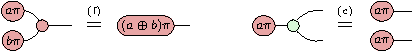
\includegraphics[width=0.7\textwidth]{chapter-2/xor_copy}
    \caption{XOR gate (left) and COPY gate (right) with respect to the $Z$ eigenstates.}
    \label{xor}
    \label{copy}
\end{figure}

Using the natural commutation relation of the classical XOR and COPY gates, we define the \textit{bialgebra rule} (\textit{ba}). We encourage the reader to verify this relation.

\begin{figure}[H]
    \centering
    \includezxdiagram{chapter-2/bialgebra}{1}
    \caption{The bialgebra rule (and its classical motivation).}
    \label{bialgebra}
\end{figure}

%%%

\subsection{Hopf Rule}

Like with the bialgebra rule, our motivation for this rule stems from the behaviour of the classical XOR and COPY gates. Since copying two bits then taking their XOR invariably yields 0, we can define the \textit{Hopf rule} (\textit{hpf}).

\begin{figure}[H]
    \centering
    \includezxdiagram{chapter-2/hopf}{1}
    \caption{The Hopf rule (and its classical motivation).}
    \label{hopf}
\end{figure}

%%%

\newpage
\section{Conjugating with Paulis and Cliffords}

In this section we will develop several results later used in this thesis.
- Pauli Y gate
- conjugation by XPlus and XMinus
- conjugation by hadamards
- refer to zxfermion

Next, using the $\pi$ copy rule (\ref{pi-copy}), we can show that conjugating a $Z$ rotation by Pauli $X$ gates, negates the phase of the rotation, $\alpha \rightarrow -\alpha$.

\includezxdiagram{chapter-4/phase_flip}{0.7}


% PAULI GADGETS
\chapter{\label{pauli-gadgets}Pauli Gadgets}

A Pauli string $P$ is defined as a tensor product of the members of the Pauli group $P \in \{I, Y, Z, X\}^{\otimes n}$, where each Pauli operator acts on a distinct qubit (indicated by the subscript). Note that the Pauli matrices are Hermitian operators, and therefore, so are Pauli strings. For convenience, we will drop the subscripts.

\includezxdiagramtext{chapter-3/pauli_string}{0.22}
{I_0 \,\, Z_1 \, X_2 = I \otimes Z \otimes X}

\textit{Stone's Theorem} \cite{Stone1932} states that a strongly continuous one parameter unitary group $U(\theta)$ is generated by a Hermitian operator, $P$.
\begin{equation*}
    U(\theta) = e^{i\theta P} = 1 + i\theta P +
    \frac{1}{2} [i\theta P]^2 +
    \frac{1}{6} [i\theta P]^3 + \dots
\end{equation*}

There is therefore a one-to-one correspondence between Hermitian operators and one parameter unitary groups \cite{Yeung2020}. The time evolution of a quantum mechanical system, described by the Hamiltonian $H$, is defined by the one parameter unitary group $e^{itH}$, whilst arbitrary rotation gates in the $Z$, $X$ and $Y$ bases are described by the one parameter unitary groups of the Pauli matrices $Z$, $X$ and $Y$.
\begin{equation*}
    R_Z(\theta) = e^{i\frac{\theta}{2} Z} \qquad
    R_Y(\theta) = e^{i\frac{\theta}{2} Y} \qquad
    R_X(\theta) = e^{i\frac{\theta}{2} X}
\end{equation*}

Phase gadgets are defied as the one parameter unitary groups of Pauli strings consisting of the $I$ and $Z$ matrices, $P \in \{I, Z\}^{\otimes n}$.
\begin{equation*}
    \Phi(\theta) = \text{exp} \left[
    i\frac{\theta}{2} (I \otimes Z \otimes Z \otimes \dots)
    \right]
\end{equation*}

In quantum circuit notation, phase gadgets are represented by a layer of CNOTs followed by a rotation in the $Z$ basis, followed by another layer of CNOTS.

\includezxdiagramtext{chapter-3/phase_gadget_expanded}{0.35}
{\text{exp} \left( i \frac{\theta}{2} Z \otimes Z \otimes Z \right)}

The first layer of CNOTs can be thought of as computing the parity of the input qubits by creating an entangled state. The rotation in the $Z$ basis then rotates the entangled state by $e^{i\theta/2}$ or $e^{-i\theta/2}$, depending on its parity. The final layer of CNOTs can be thought of as uncomputing the parity. Since phase gadgets correspond to diagonal unitary matrices in the $Z$ basis, they apply a global phase to a given state without changing the distribution of the observed state \cite{Yeung2020}.

There are many equivalent ways of expressing the same phase gadget in terms of CNOT gates and $Z$ rotation gates. Furthermore, the diagonal action of phase gadgets suggests that a more symmetrical structure exists for phase gadgets in the ZX calculus.

Indeed, we find that by iteratively applying the bialgebra rule, we can represent phase gadgets as follows.

\includeZxEqZxEq{chapter-3/ZIZ}{0.19}
{=\, \text{exp} \left( i \frac{\theta}{2} Z \otimes I \otimes Z \right)}
{chapter-3/ZZZ}{0.19}
{=\, \text{exp} \left( i \frac{\theta}{2} Z \otimes Z \otimes Z \right)}

By deforming our diagram \textit{d} and using the spider fusion \textit{f} (\ref{spider-fusion}), identity \textit{id} (\ref{identity}) and bialgebra \textit{ba} (\ref{bialgebra}) rules, we are able to show the correspondence between phase gadgets in normal quantum circuit form and in their form in the ZX calculus.

\includezxdiagram{chapter-3/phase_gadget_proof}{0.85}

It is then a simple matter of recursively applying this proof to phase gadgets in quantum circuit form to generalise it to arbitrary arity phase gadgets.

\includezxdiagram{chapter-3/phase_gadget_proof2}{1}

\section{Phase Gadgets}%
\label{phase-gadgets}

Phase gadgets are defined as the one parameter unitary groups of Pauli strings consisting of only the Pauli $I$ and $Z$ matrices, $P \in \{I, Z\}^{\otimes n}$. They can be naively implemented as a $Z$ rotation nested between two ladders of CNOT gates.

\includezxdiagramtext{chapter-3/phase_gadget_expanded}{0.28}
{\text{exp} \left( - i \frac{\theta}{2} Z \otimes Z \otimes Z \right)}

Phase gadgets correspond to unitary maps which are diagonal in the $Z$ computational basis \cite{Cowtan2020}. Consequently, they apply a global phase to a state without changing the distribution of the observed state \cite{Yeung2020}. Phase gadgets have the following representation in the ZX calculus.

\includezxdiagramtext{chapter-3/phase_gadget}{0.15}{
\text{exp} \left( - i \frac{\theta}{2} Z \otimes Z \otimes Z \right)}

Using the identity (\ref{identity}), spider fusion (\ref{spider-fusion}) and bialgebra (\ref{bialgebra}) rules, we are able to derive its representation in the ZX calculus.

\begin{figure}[H]
    \centering
    \includezxdiagram{chapter-3/phase_gadget_proof}{0.75}
    \caption{Phase gadget result.}
    \label{phase-gadget-result}
\end{figure}

It is then a simple matter of recursively applying this result to phase gadgets in quantum circuit notation to generalise to arbitrary arity.

\includezxdiagram{chapter-3/phase_gadget_proof2}{0.8}%

Phase gadgets can be interpreted as first copying each input in the $Z$ basis (\ref{copy}), computing the parity of the state by taking the XOR (\ref{xor}), then multiplying the state by $\text{exp} \left(-i\frac{\theta}{2} \right)$ or $\text{exp} \left(i\frac{\theta}{2} \right)$ depending on its parity \cite{Yeung2020}. 

\includezxdiagramtext{chapter-3/phase_gadget_interpretation}{0.2}{
\quad\text{diag} \left\{
\begin{pmatrix}
    1 \\ e^{i\theta} \\ e^{i\theta} \\ 1 \\
    e^{i\theta} \\ 1 \\ 1 \\ e^{i\theta}
\end{pmatrix} \cdot e^{-i\frac{\theta}{2}}
\right\}
}

%%%

\subsubsection{Phase Gadget Identity}%

We can show that phase gadgets with an angle $\theta = 0$ are equivalent to identity using the state copy (\ref{state-copy}), spider fusion (\ref{spider-fusion}) and identity (\ref{identity}) rules.

\includezxdiagram{chapter-3/phase_gadget_identity}{0.8}

%%%

\subsubsection{Phase Gadget Fusion}%
\label{phase-gadget-fusion}
We can show that phase gadgets with the same distribution of legs fuse together and their phases add using the spider fusion (\ref{spider-fusion}) and bialgebra (\ref{bialgebra}) rules.

\includezxdiagram{chapter-3/phase_gadget_fusion_steps}{0.8}

%%%

\subsubsection{Phase Gadget Commutation}%
\label{phase-gadget-commutation}

Phase gadgets can be shown to commute using the spider fusion rule (\ref{spider-fusion}).

\includezxdiagram{chapter-3/phase_gadget_commutation}{0.6}

%%%

\subsubsection{Phase Gadget Decomposition}%

Using the phase gadget result described above (\ref{phase-gadget-result}), we can show that a two-legged phase gadget can be decomposed in the following two ways.

\begin{figure}[H]
    \centering
    \includezxdiagram{chapter-3/phase_gadget_decomposition1}{0.6}
    \caption{Phase gadget decomposition result.}
    \label{phase-gadget-decomposition}
\end{figure}

\subsubsection{Balanced Tree Representation}%
By recursively applying this decomposition, we can demonstrate that a phase gadget in the balanced tree representation can achieve a circuit depth of $2\text{log}_2(n) + 1$, rather than $2n - 1$ as in the ladder representation, where $n$ is the number of qubits \cite{Cowtan2019}.

\begin{figure}[H]
    \centering
    \includezxdiagram{chapter-3/phase_gadget_decomposition}{0.95}
    \caption{Phase gadget in the balanced tree representation.}
    \label{balanced-tree}
\end{figure}

\subsubsection{Single-Legged Phase Gadgets}
Single-legged phase gadgets simply correspond to $Z$ rotations. Therefore, phase gadgets can be thought of as the many-qubit generalisation of $Z$ rotations.

\begin{figure}[H]
    \centering
    \includezxdiagram{chapter-3/phase_gadget_single_leg_steps}{0.5}
    \caption{Single-legged phase gadget as a $Z$ rotation.}
    \label{phase-gadget-single-leg}
\end{figure}


\section{Pauli Gadgets}

Pauli gadgets are defined as the one parameter unitary groups of Pauli strings in the set $\{I, X, Y, Z\}^{\otimes n}$. By performing a Clifford conjugation (\ref{clifford-conjugation}) on the legs of a phase gadget, we obtain the corresponding Pauli gadget. That is, Pauli gadgets are phase gadgets associated with a change of basis. Hence, whilst phase gadgets alone cannot alter the distribution of the observed state, Pauli gadgets can \cite{Yeung2020}. 

\includezxdiagramtext{chapter-3/pauli_gadget}{0.6}{
\text{exp} \left( - i \frac{\theta}{2}
Y \otimes Z \otimes X \right)}

Pauli gadgets come equipped with a similar set of rules to phase gadgets that describe their interactions with other gadgets. For instance, adjacent Pauli gadgets with \textit{matching legs} fuse, and their phases add modulo $2\pi$.

\begin{figure}[H]
    \centering
    \includezxdiagram{chapter-3/pauli_gadget_fusion}{0.6}
    \caption{Pauli gadget fusion rule.}
    \label{pauli-gadget-fusion}
\end{figure}

Similar to the phase gadget commutation rule (\ref{phase-gadget-commutation}), we have that adjacent Pauli gadgets with \textit{no mismatching legs} commute.

\begin{figure}[H]
    \centering
    \includezxdiagram{chapter-3/pauli_gadget_commutation}{0.7}
    \caption{Pauli gadget commutation rule.}
    \label{pauli-gadget-commutation}
\end{figure}

Single-legged Pauli gadgets correspond to rotations in their respective basis.

\vspace{5pt}
\includezxdiagram{chapter-3/pauli_gadget_single_leg}{0.8}



% COMMUTATION RELATIONS
\chapter{Controlled Rotations}%
\label{controlled-rotations}

Controlled rotations play an important part in UCC ansätze representing fermionic systems. They can be used to account for the fermionic antisymmetry observed in fermionic systems by applying a phase (rotation) depending on the parity of the state. In other words, the rotation is \textit{controlled} by the parity of the state.

In this chapter, we will first discuss the form of singly-controlled rotations, as in Yeung \cite{Yeung2020}, and later show how these can be used to construct higher order controlled rotations, using the ZX calculus. We will later use the results derived in this chapter to demonstrate the correspondence between excitation operators and controlled rotations in Chapter \ref{excitation-operators}.

\section{CNOT Commutation}

When a CNOT gate is \textit{pushed} through a Pauli gadget, it modifies its legs. That is, the resulting gadget is defined by a new Pauli string. We have already encountered this when decomposing phase gadgets (\ref{phase-gadget-proof}) using the bialgebra rule (\ref{bialgebra}).

\includezxdiagram{chapter-4/phase_gadget_decomposition}{0.6}

Above, we have inserted two adjacent CNOTs (self-inverse), then pushed one of them through the phase gadget. We can say that a CNOT gate `commutes' through a $\text{exp} [i\frac{\theta}{2} (Z \otimes Z)]$ gadget yielding a $\text{exp} [i\frac{\theta}{2} (I \otimes Z)]$ gadget.

\includezxdiagram{chapter-4/CNOT_ZZ_IZ}{0.7}

The ZX calculus can be used to identify how CNOT gates commute through any Pauli gadget. Note that the following examples are not exhaustive -- there are 16 possible permutations with repetition of $\{I, X, Y, Z\}$ taken two at a time.

\includezxdiagram{chapter-4/CNOT_examples}{0.8}

In practice, it may be tedious to use the bialgebra and other rules to identify each commutation relation. There exists, however, a simple trick for identifying these relations. The CNOT gate belongs to the Clifford group $C$. That is, the set of transformations that normalise the Pauli group. For instance, conjugating the Pauli $X$ gate with the Hadamard $H$ (where $H \in C$), yields the $Z$ gate.
\begin{equation*}
    Z = HXH
\end{equation*}
Recall that Pauli gadgets are defined as the one parameter unitary groups of a given Pauli string $P$, where $P \in \{I, Z, X, Y\}^{\otimes n}$. It can be shown, through the relevant Taylor expansion, that conjugating a Pauli gadget is equivalent to finding the one parameter unitary group of the conjugated Pauli string (see Appendix \ref{conjugation}). In other words, if we can determine the behaviour of a pair of Paulis with the CNOT gate, we can know the behaviour of the corresponding gadget.

Let us first derive the phase gadget decomposition commutation relation (\ref{phase-gadget-proof}). We first express two Pauli $Z$ gates as $Z$ rotations. We then push the bottom Pauli through the CNOT target (red $X$ spider) using the $\pi$ copy rule (\ref{pi-copy}). We can then push the top Pauli through the CNOT control using the spider fusion rule (\ref{spider-fusion}) to cancel one of the copied Pauli $Z$ gates obtaining the same relation as before.

\includezxdiagram{chapter-4/commutation_trick}{0.7}

Up to a global phase of $-i$ (CHECK), the Pauli Y gate can be expressed as a Pauli X gate followed by a Pauli Z gate. We will use this to identify how the CNOT gate interacts with a $\text{exp} [i\frac{\theta}{2} (X \otimes Y)]$ gadget.

\includezxdiagram{chapter-4/commutation_trick_YX}{1}

Using this method, we are able to derive all CNOT commutation relations (see Appendix \ref{cnot_commutations} for the complete set of CNOT commutation relations).

\section{Clifford Commutation}


% ZX FERMION SOFTWARE
\chapter{Excitation Operators}%
\label{excitation-operators}

In this chapter, we will use the theory that we have developed in Chapter \ref{pauli-gadgets} on Pauli gadgets and their commutation relations, and in Chapter \ref{controlled-rotations} on controlled rotations, to study the excitation operators used to construct Unitary-Product State ansätze.


\begin{itemize}[itemsep=-5pt]
    \item show example UCC ansatz in introduction using 'box' notation
    \item show commutation relations between different excitation operators
    \item introduce conjugation by some clifford to yield phase polynomial and suggest optimisation from \cite{Cowtan2020}
    \item \textbf{optimisations section} -- show balanced tree representation stuff "Circuit optimisation is typically carried out by pattern replacement: recognising a subcircuit of specific form and replacing it with an equivalent" \cite{Cowtan2019}
    \item "In principle, local rewriting of gate sequences is sufficient for any circuit optimisation3. However, in practice, good results often require manipulation of large-scale structures in the quantum circuit. Phase gadgets are one such macroscopic structure that is easy to identify within circuits, easy to synthesise back into a circuit, and have a useful algebra of interactions with one another." \cite{Cowtan2019}
    \item "Further, in the balanced tree form more of the CX gates are “exposed” to the rest of the circuit, and could potentially be eliminated by a later optimisation pass" \cite{Cowtan2019}
\end{itemize}

\section{Creating Gadgets}

\section{Creating Circuits}

\section{Manipulating Circuits}

The \lstinline{GadgetCircuit} class comes equipped with the \lstinline{apply()} method that allows us to insert a cancelling gate pair into the circuit, hence the \lstinline{apply()} method \textit{does not} modify the matrix corresponding to the circuit. The first parameter specifies the quantum gate that we want to apply, whilst the \lstinline{start} and \lstinline{end} parameters allow us specify the positions to insert at. 

\includejupyter{chapter-5/apply1}{chapter-5/apply1_zx}{0.4}

If we choose not to specify the \lstinline{start} and \lstinline{end} parameters, one gate is inserted at the start, and the other, at end of the circuit. The \lstinline{GadgetCircuit} class then handles the relevant CNOT-gadget commutation relations, yielding the expected gadget.

\includejupyter{chapter-5/apply2}{chapter-5/apply2_zx}{0.4}

WE COULD HAVE CHOSEN AN XXX GADGET, or indeed any other gadet. This functionality is built of top of Stim's stabiliser circuit / clifford tableau functionality applied to a Pauli string. [insert short explanation about clifford tableau]. Alternatively, we could have chosen any other clifford (CZ, ZPlus, etc) to form the clifford tableau.

\includejupyter{chapter-5/apply_cz}{chapter-5/apply_cz_zx}{0.45}

We can use the \lstinline{GadgetCircuit} class to manipulate circuits consisting of multiple gadgets simultaneously. Consider the following circuit in which we have instantiated a paired double excitation operator as a \lstinline{GadgetCircuit} object.

GIVE EXAMPLES

\includejupyter{chapter-5/double1}{chapter-5/double1_zx}{0.8}

Then by applying three pairs of CNOTs to all the gadgets in the circuit, we obtain the following equivalent circuit.

\includejupyter{chapter-5/double2}{chapter-5/double2_zx}{0.84}


\chapter{ZxFermion Software}%
\label{zxfermion}

Visit \textbf{\href{https://github.com/aymannel/zxfermion}{github.com/aymannel/zxfermion} }for complete documentation.

Motivated by the need for an accessible tool to explore research ideas related to circuits of Pauli gadgets, we decided to build the ZxFermion Python package for the visualisation and manipulation of circuits of Pauli gadgets. It is built on top of the PyZX \lstinline{BaseGraph} API \cite{Kissinger2020} and the Stim \lstinline{Tableau} class \cite{Gidney2021}.

ZxFermion provides classes to represent Pauli gadgets and common quantum gates and encodes the commutation relations developed in Section \ref{clifford-commutation-relations}. It is designed to integrate within Jupyter notebook environments, enabling users to generate interactive ZX diagrams directly in the output cell. ZxFermion offers an accessible tool for studying the interactions of Pauli gadgets in the context of VQE.

Using ZxFermion, we can replicate all of the commutation relations described in Section \ref{commutation-relations} as well as the proofs discussed in Chapter \ref{excitation-operators}, showcasing a noticeable acceleration in research pace. We anticipate that both chemists and computer scientists exploring quantum computing within the VQE framework will find this software tool useful.


\section{Controlled-Rotations}

\subsection{Singly-Controlled Rotations}
Singly-controlled Z rotation.

\begin{figure}[hb]
    \centering
    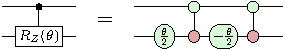
\includegraphics[width=\textwidth]{chapter-4/CRZ}
    % \caption{}
    % \label{}
\end{figure}

Singly-controlled X and Y rotations obtained by conjugating the control qubit.

\begin{figure}[hb]
    \centering
    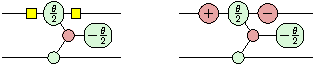
\includegraphics[width=0.6\textwidth]{chapter-4/CRX_CRY}
    % \caption{}
    % \label{}
\end{figure}

\subsection{Doubly-Controlled Rotations}
hello world


\subsection{Triply-Controlled Rotations}
hello world
hello world



\chapter{\label{conclusion}Conclusion}

\section{Conclusion}

\section{Future Work}



%%% ========== APPENDICIES  ========== %%%

\startappendices
\subsection{Hadamard}%
\label{appendix-hadamard}

Below are several equivalent definitions of the Hadamard generator. Note that the two rightmost definitions do not require any scalar correction.

\begin{figure}[H]
\centering
    \centering
    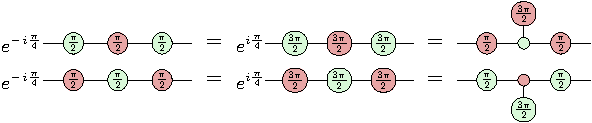
\includegraphics[width=1\textwidth]{chapter-2/hadamard_decomp}
    \caption{Equivalent definitions of the Hadamard generator.}
\end{figure}

%%%

\subsection{Phase Gadgets}%
\label{appendix-phase-gadget-fusion}

We can show how two adjacent phase gadgets fuse using the spider fusion (\ref{spider-fusion}) and bialgebra (\ref{bialgebra}) rules as follows.

\includezxdiagram{chapter-3/phase_gadget_fusion_steps}{0.8}%

%%%

\subsection{Clifford Conjugation Stuff}%
\label{conjugation}

\begin{align*}
    Ce^PC^\dagger &= C \sum_{n=0}^\infty \brac{P^n}{n!} C^\dagger \\
    CP^nC^\dagger &= \sum_{n=0}^\infty \frac{C P^n C^\dagger}{n!} \\
    CP^nC^\dagger &= \sum_{n=0}^\infty \frac{(C P C^\dagger)^n}{n!} \\
    CP^nC^\dagger &= (CPC^\dagger)^n
\end{align*}

%%%

\subsection{CNOT Commutation Relations}

\begin{figure}[H]
    \centering
    \includezxdiagram{chapter-3/cnot_commutations}{1}
    \caption{Complete set of CNOT commutation relations.}
    \label{cnot_commutations}
\end{figure}

\subsection{General One-Body Excitation Operator}%
\label{appendix-one-body-general}

\includezxdiagram{chapter-5/one_body_general_proof}{1}



%%% ========== REFERENCES ========== %%%
\setlength{\baselineskip}{0pt}

{\renewcommand*\MakeUppercase[1]{#1}%
\bibliography{references}{}

\end{document}
